\chapter*{Introducción}
\addcontentsline{toc}{section}{Introducción}

La reescritura es una técnica que consiste en reemplazar términos de
una expresión con términos equivalentes. Por ejemplo, dadas las reglas
$x * 0 \Rightarrow 0$ y $x + 0 \Rightarrow 0$ pueden usarse para
simplificar la siguiente expresión:

\[
x + (\underline{x*0}) \longrightarrow \underline{x + 0} \longrightarrow x
\]

Pero no sólo se puede aplicar para ecuaciones. Se puede usar para
demostrar enunciados. Por ejemplo, dadas las reglas
$s(M) \leq s(N) \Rightarrow M \leq N$ y
$0 \leq N \Rightarrow \texttt{True}$ pueden aplicarse a:

\[
  s(0) \leq s(x) \longrightarrow 0 \leq s(x) \longrightarrow
  \texttt{True}
\]

Donde $s(x)$ es la función sucesor de $x$.

En definitiva, podemos aplicar reescritura a cualquier tipo de
expresión (ya sea lógica, ecuacional, etc) siempre y cuando se pueda
hacer una sustitución. Esta sustitución se hace de término a término.

Sin embargo, debemos formalizar qué entendemos por término. Un término
estará construido por variables, símbolos constantes y símbolos de
funciones. Al estar constituidos por funciones, una representación
natural de los términos se realiza mediante árboles. Por ejemplo el
término $f(i(e),f(x,e))$ se representa como,

\begin{figure}[h]
  \centering
  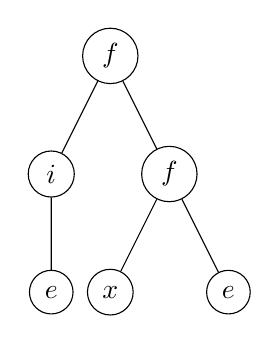
\begin{tikzpicture}
    \node [circle,draw]{$f$} child {node
      [circle,draw]{$i$}
        child{node[circle,draw]{$e$}}} child {node
      [circle,draw]{$f$} child {node
        [circle,draw]{$x$}} child {node
        [circle,draw]{$e$}} };
  \end{tikzpicture}
\end{figure}

Donde $i,f$ representa un símbolo de función de aridad 1 y 2
respectivamente, $e$ representa un símbolo constante y $x$ representa
una variable.

Los anteriores ejemplos también se pueden escribir como términos,

\[
  \begin{array}{rcl}
    x +(x*0) & \longrightarrow  & +(x,*(x,0)) \\ \\
    s(0) \leq s(x) & \longrightarrow & \leq(s(0),s(x)) \\ \\

  \end{array} 
\]

Un sistema de reescritura de términos es un conjunto de sustituciones
término a término. A estas sustituciones las llamaremos reglas.

Estos conjuntos de reglas determinan ciertas propiedades según los
elementos que contengan. Por ejemplo,

\begin{figure}[h]
  \centering
  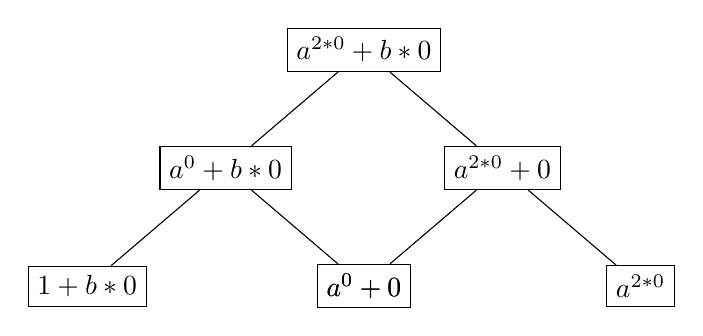
\begin{tikzpicture}[sibling distance=10em]
    \node [draw]{$a^{2*0} + b*0$}
    child {
      node[draw]{$a^0 + b*0$}
      child{node[draw]{$1 + b*0$}}
      child{node[draw]{$a^0 + 0$}}
      }
      child {
        node [draw]{$a^{2*0} + 0$}
        child {node [draw]{$a^0 + 0$}}
        child {node [draw]{$a^{2*0}$}} };
  \end{tikzpicture}
\end{figure}

Este diagrama de árbol representa para cada rama una aplicación de las
distintas reglas. Podemos hacernos dos preguntas fundamentales, si
este árbol será finito y si todas las hojas son la misma; es decir,
siguiendo cualquier rama, llegar hasta el mismo término. Estas dos
preguntas son los principales problemas de la reescritura.

Analizar si este árbol es finito es equivalente a preguntarse si en
algún momento podemos dejar de aplicar las reglas. Por ejemplo, para
el término $s(1) + s(0)$ y para la regla $s(3) \Rightarrow 4$, no
podemos seguir sustituyendo términos, por tanto diremos que el sistema
termina.

Es importante observar que no siempre tener un mayor número de reglas
es mejor. Por ejemplo, para las reglas $ x + 0 \Rightarrow x$ y
$x \Rightarrow x + 0$;

\[
  x + 0 \longrightarrow x \longrightarrow x+0 \longrightarrow \dots
\]

Otro de los problemas que tenemos que tratar es el de ver si el árbol
termina en una misma hoja. Si esta situación ocurre en nuestro sistema
diremos que es confluente.

Para analizar si un sistema es confluente o no debemos estudiar el
momento en el que se crea una ramificación del árbol. La idea
intuitiva es ver si la sustitución que se hace en cada rama se solapa
entre sí. A estos puntos los llamaremos pares críticos

También podemos modificar el conjunto reglas de los reescritura para
que se verifiquen estas dos propiedades. A este proceso se le llama
completación. Los cambios que se realizan al conjunto de reglas van
desde eliminar alguna regla, hasta añadir propias.

Como es de esperar, el algoritmo de completación debe tener en cuenta
los pares críticos. Una primera idea de implementación sería modificar
las reglas hasta no tener ningún par crítico.

Sin embargo el cálculo de pares críticos es muy costoso si hablamos de
grandes sistemas de reescritura. Por ello introduciremos el algoritmo
de Huet, que pese a usar pares críticos en el proceso, reduce la
cantidad de cálculos a realizar.

A continuación, describiré brevemente los contenidos de cada capítulo.

En el capítulo 1, introduciremos los sistemas de reducción abstractos y
definiremos algunas de sus características fundamentales, algunas de
ellas se volverán a tratar con mayor profundidad en capítulos
posteriores.

En el capítulo 2, estudiaremos las definiciones de términos y
sustituciones, así como sus características. Además, relacionando
términos y sustituciones, daremos una caracterización de
$\xleftrightarrow{*}$,

En el capítulo 3, formalizaremos la definición de sistema de
reescritura de términos y estudiaremos el problema de unificación para
términos.

En el capítulo 4, resolveremos el problema de decidir si un sistema de
reescritura es terminante. Veremos que, en general, el problema es
indecidible. Por ello, le daremos varios enfoques según las
propiedades que tenga el sistema para poder decidir la terminación.

En el capítulo 5, estudiaremos la confluencia para los sistemas de
reescritura. Probaremos que el problema de decidir si un sistema es
confluente es indecidible. Sin embargo, a partir del estudio de pares
críticos y ortogonalidad, podremos dar varios resultados sobre la
confluencia.

Por último, en el capítulo 6, enunciaremos dos algoritmos de
completación. Para ambos, estudiaremos su funcionamiento y si son
correctos.

%%% Local Variables:
%%% mode: latex
%%% TeX-master: "SRT_en_Haskell"
%%% End:
